\documentclass[a4paper]{article}
\usepackage[utf8]{inputenc}
\usepackage{amsmath}
\usepackage{polski}
\usepackage[polish]{babel}
\usepackage[T1]{fontenc}
\usepackage[a4paper,top=3cm,bottom=2cm,left=3cm,right=3cm,marginparwidth=1.75cm]{geometry}
\usepackage{graphicx}
\usepackage{float}
\usepackage{longtable}
\usepackage{pdflscape}
\usepackage[backend=bibtex]{biblatex}
\graphicspath{{../img/}}

\title{Optymalizacja fabryki z wykorzystaniem algorytmu immunologicznego (selekcji klonalnej)}
\author{Artur Bauer \and Kamil Szostek \and Sławomir Goździewski \and Wiktor Filipiak}
\date{\today}

\usepackage[pdftex,
            pdfauthor={Artur Bauer \& Kamil Szostek \& Sławomir Goździewski \& Wiktor Filipiak},
            pdftitle={\@title},
            pdfsubject={Glebokie uczenie i inteligencja obliczeniowa},
            pdfkeywords={Automatyka i Robotyka},
            pdfproducer={Latex},
            pdfcreator={pdflatex}]{hyperref}

\bibliography{citations.bib}

\begin{document}
%--------------------------------------------------------%
%	COVER PAGE
%--------------------------------------------------------%

\begin{titlepage}
\makeatletter

  \newcommand{\HRule}{\rule{\linewidth}{0.5mm}} % Defines a new command for the horizontal lines, change thickness here

  \center % Center everything on the page


%	HEADING SECTION

  \textsc{\LARGE Akademia Górniczo-Hutnicza}\\[1.5cm] % Name of your university/college
  \textsc{\Large  Głębokie uczenie i inteligencja obliczeniowa }\\[0.5cm] % Major heading such as course name
  \textsc{\large Automatyka i Robotyka II Stopień}\\[0.5cm] % Minor heading such as course title
  \textsc{2019/2020}\\[0.5cm] % Minor heading such as course title

%	TITLE SECTION

  \vspace{1.5 cm}
  \HRule \\[0.4cm]
  { \huge \bfseries \@title} \\[0.4cm] % Title of your document
  \HRule \\[1.5cm]
 
%	AUTHOR SECTION

  {\em\Large\textbf Skład zespołu:}\\
  \vspace{.5 cm}
    Artur Bauer\\
    Kamil Szostek\\
    Sławomir Goździewski\\
    Wiktor Filipiak
  \vspace{1.5 cm}
  
  
  {\em\Large\textbf Opiekun:}\\
  \vspace{.5 cm}
  dr hab. inż. Joanna Kwiecień
  
%	DATE SECTION

  \vspace{1.5 cm}
  {\large Złożono: \@date}\\[3cm] % Date, change the \today to a set date if you want to be precise


\vfill % Fill the rest of the page with whitespace

\end{titlepage}

%-----------------------------------------------------------------

\newpage

\tableofcontents

\newpage
\section{Wstęp}
\subsection{Factory model}\label{factory}

\begin{figure}[ht]
\centering
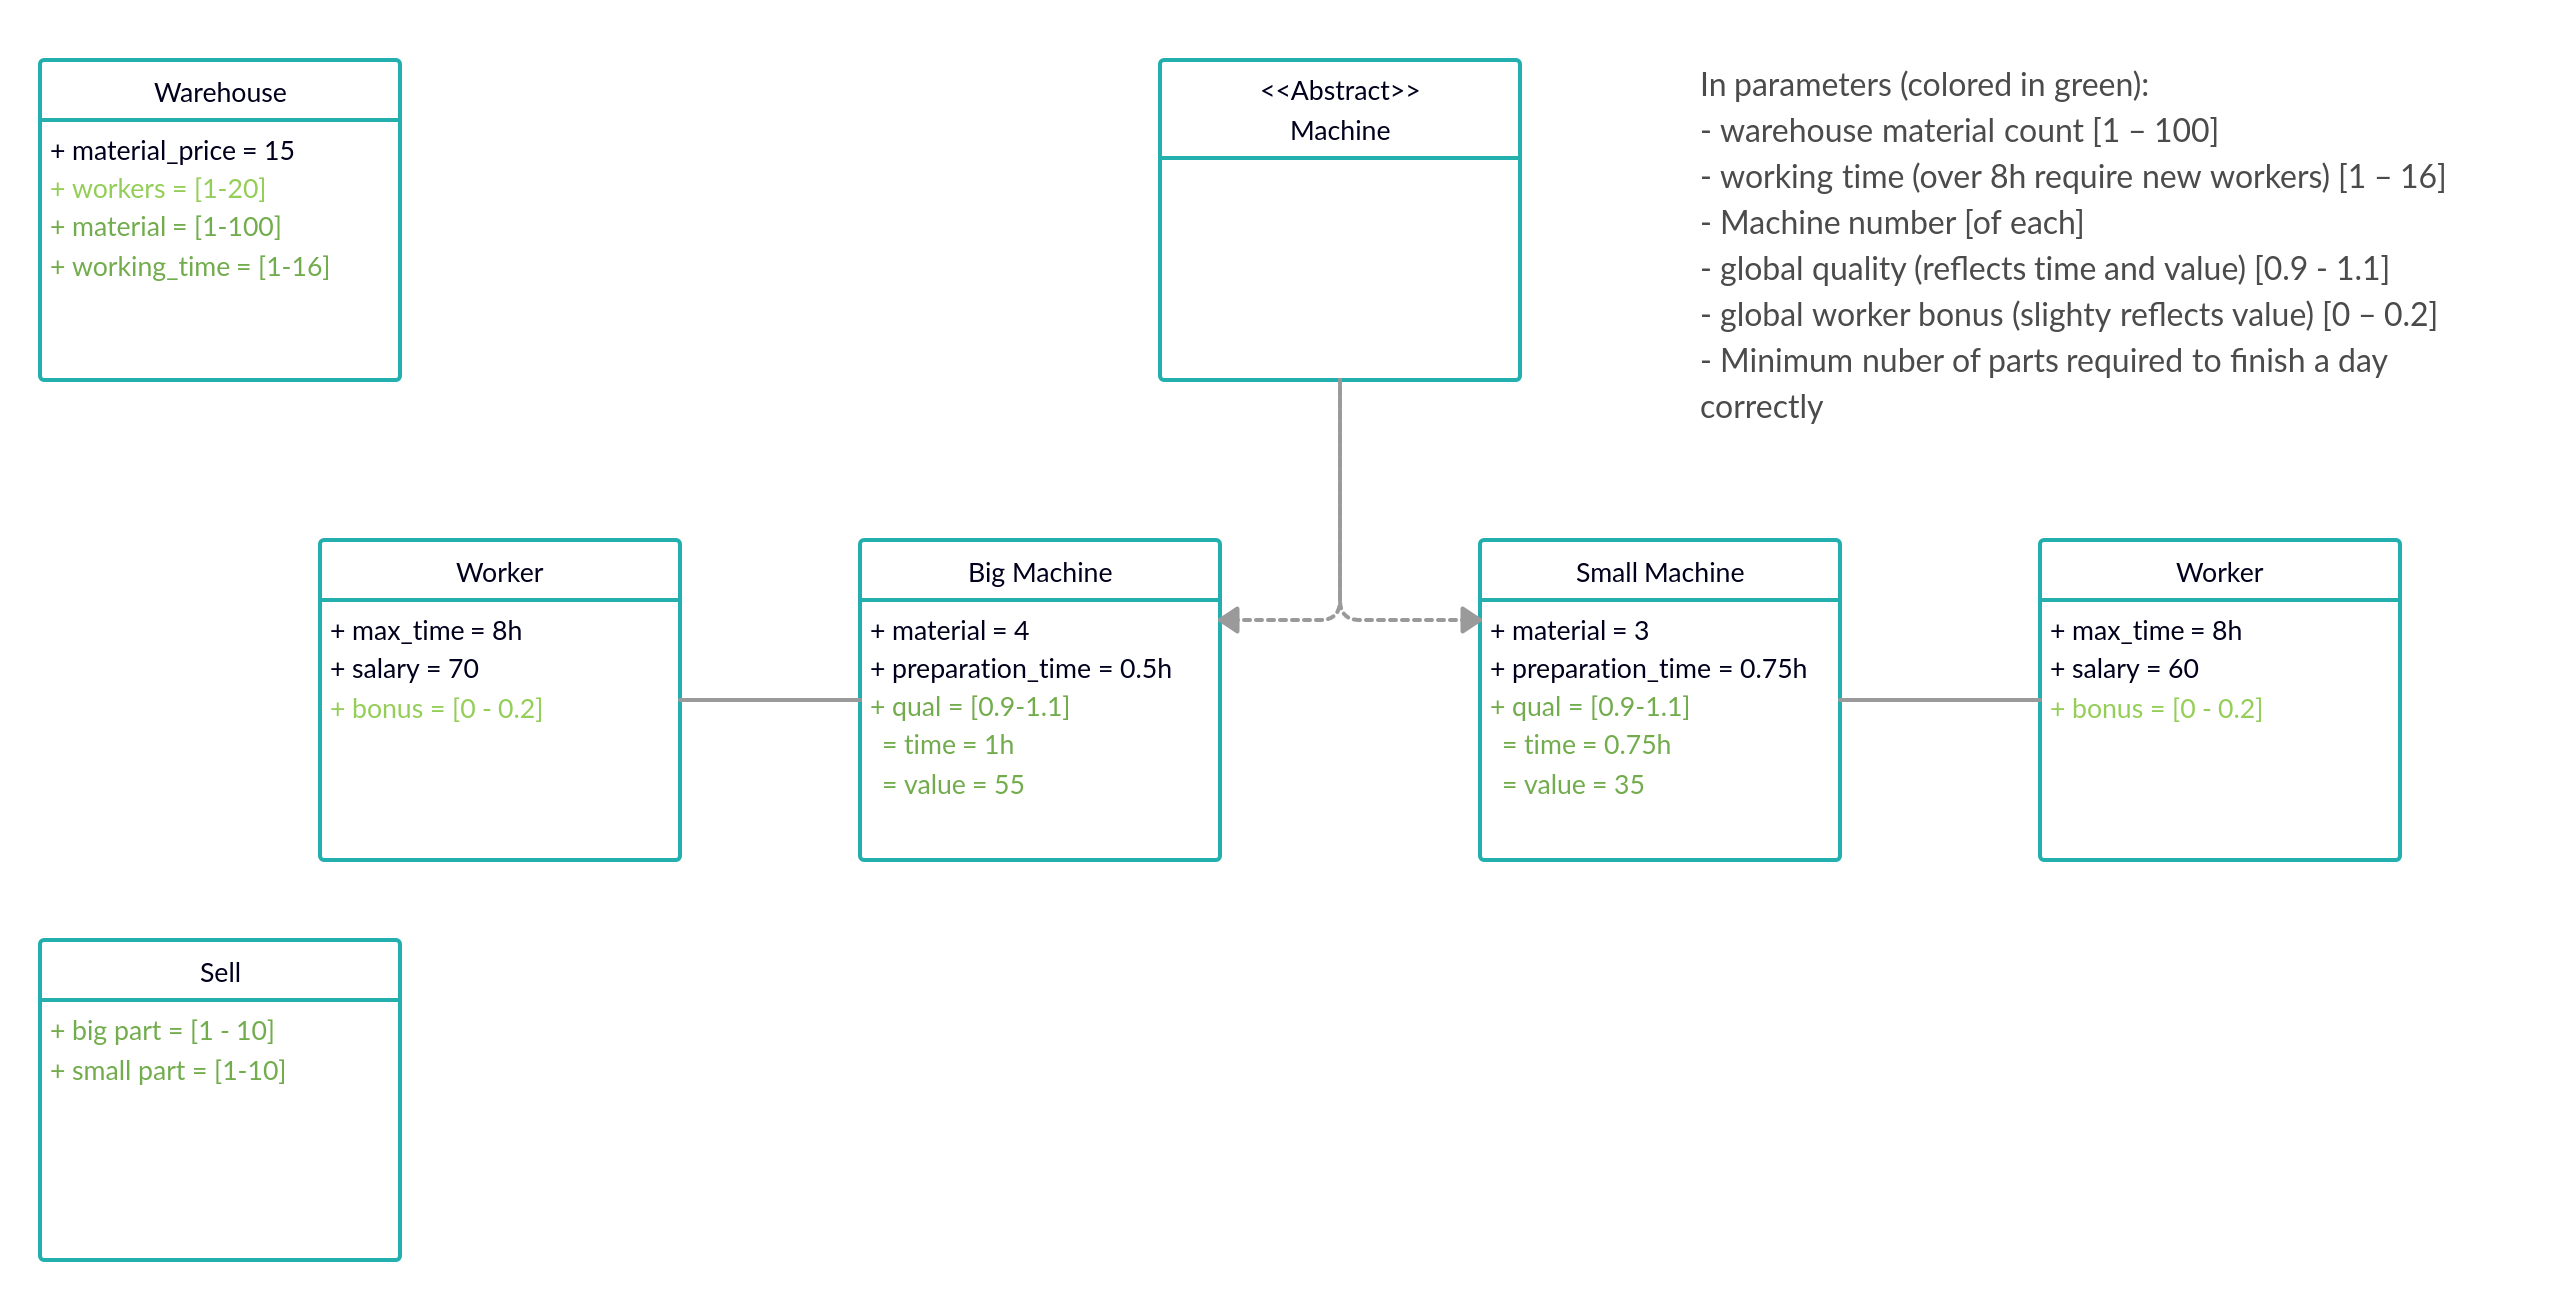
\includegraphics[width=.7\textwidth]{Factory_scheme.png}
\caption{Factory scheme}
\end{figure}

\subsubsection{Factory main goal function:}\label{factory-main-goal-function}

$$Income = \sum^{n_p}_{i=1}(p_i*(v_i-m_i*m_p)) - (1+b_i)*\sum^{n_w}_{i = 1}(w_i*s_i *t_{wi}) - m_r*m_p - punish$$

Where:
\begin{itemize}
    \item $n_p$ -- number of item types ( param )
    \item $p_i (n_m)$ -- number of manufactured i-type items
    \item $v_i(v_{bi}, t_{wi},t_{bi},w_q)$ -- value of the i-type items
    \item $m_i$ -- number of material needed to manufacture the i-type item ( param )
    \item $m_p$ -- material price ( param )
    \item $n_w$ -- number of types of employees ( param )\item$w_i$ -- number of i-type employees (param)
    \item $s_i$ -- the salary of i-type employees\item$b$ -- the bonus for employees (param)
    \item $t_{wi}$ -- real working time of the i-type machine/employee for one product
    \item $m_r(p_i,n_m)$ -- material remains, unused material
    \item $p_{i_{min}}$ -- minimum number of i-type items that must be manufactured to avoid punishment (param) 
    \item $p_{i_{max}}$ -- maximum number of items that can be manufactured 
    \item $n_m$ -- number of materials in the warehouse at the beginning of the day (param)
    \item $punish(p_{un}, p_{num_i}, v_i)$ -- punishment for not produced required item number
\end{itemize}
\subsubsection{Punish}
$punish = p_{un}*\sum^{n_p}_{i=1}(p_{num_i})*v_i$

$p_{num_i}= \left\{\begin{matrix} 0  \;\quad\quad\quad\quad  \textrm{if} \quad  p_{i_{min}}-p_i \leq  0    \\ p_{i_{min}}-p_i  \quad  \textrm{if} \quad  p_{i_{min}}-p_i >  0  \end{matrix}\right.$

Where: 
\begin{itemize}
    \item $p_{un}$ -- punishment rate 
    \item $p_{num_i}(p_{i_{min}}, p_i)$ -- number of i-type items for which a punishment will be charged
\end{itemize}
\subsubsection{Number of types}

Number of types of employees and machines should be the same:

$n_p = n_w$

\subsubsection{Max number of items}\label{max-number-of-items}

Numbers of i-type items must meet:

$\sum^{n_p}_{i=1} p_{i_{max}} * m_i< n_m$

\subsubsection{Real working time of the i-type machine/employee for one
product}\label{real-working-time-of-the-i-type-machineemployee-for-one-product}

$t_{wi} = t_{pi} + p_i * t_{bi}$

\subsection{Model assumption}\label{model-assumption}

\begin{longtable}[c]{lll}
Parameter & mark & value\\ \hline
Material number & $n_m$ & [$x$ - 100]\\
Material cost & $m_p$ & 15\\
Working time & ? & {[}1 - 16{]}\\
Minimal number of big parts & $p_{0_{min}}$ & [0 - 10]\\
Minimal number of small parts & $p_{1_{min}}$ & [0 -10]\\
Big machine worker salary & $s_0$ & 70\\
Big machine material requirements & $m_0$ & 4\\
Big machine preparation time & $t_{p0}$ & 30 min\\
Base big machine item value & $v_{b0}$ & 50\\
Base big machine working time per item & $t_{b0}$ & 1h\\
Number of big machines & ? & [0 - 10]\\
Small machine worker salary & $s_1$ & 60\\
Small machine material requirements & $m_1$ & 3\\
Small machine preparation time & $t_{p1}$ & 45 min\\
Base small machine item value & $v_{b1}$ & 35\\
Base small machine working time per item & $t_{b1}$ & 45 min\\
Number of small machines & ? & [0 - 10]\\
Max working time per worker & ? & 8h\\
Worker bonus & b & [0.0 - 0.2]\\
Punishment rate & $p_{un}$ & 1.5
\end{longtable}

Where:
\begin{itemize}
    \item $x$ -- number of required parts * cost of part
    \item Input parameters are given in square brackets
    \item Worker is hired on full time. Must work 8h
    \item First and second shift are equal in machine and worker count and type
    \item We reserve materials for a require items
    \item Any item manufactured over require number is a profit 
\end{itemize}


\section{Badany problem}
\subsection{Przegląd literatury}
This article is about the artificial immune system in industrial application. Basing on cutting parameters (force, vibrations, torque etc.) they try to detect tool brake using a negative-selection algorithm \cite{dasgupta1999artificial}.



This article is about the artificial immune system in industrial application. Authors compare AIS with Social Learning Mechanisms to few others AIS which use cloning alghoritm. Basing on proportional–/integral–/derivative-time they try to tune a PID \cite{wang_artificial_2017}.


\newpage
\printbibliography

\end{document}
